\documentclass[12pt,a4paper]{article}
\usepackage[legalpaper, portrait, margin=2cm]{geometry}
\usepackage[export]{adjustbox}
\usepackage{amsmath}
\usepackage{fancyhdr}
\usepackage{hyperref}
\usepackage{listings}
\usepackage{xcolor}
\usepackage{setspace}
\usepackage{enumitem}
\newcommand{\subscript}[2]{$#1 _ #2$}

\onehalfspacing

\graphicspath{ {./docs/} }

\hypersetup{
	citecolor=blue,
	colorlinks=true,
	filecolor=magenta,
	linkcolor=blue,
	pdfpagemode=FullScreen,
	pdftitle={Homework I - Group 67},
	urlcolor=blue,
}

\definecolor{codegreen}{rgb}{0,0.6,0}
\definecolor{codegray}{rgb}{0.5,0.5,0.5}
\definecolor{codepurple}{rgb}{0.58,0,0.82}
\definecolor{backcolour}{rgb}{0.95,0.95,0.92}

\lstdefinestyle{Python}{
	basicstyle=\ttfamily\footnotesize,
	breakatwhitespace=false,
	breaklines=true,
	captionpos=b,
	commentstyle=\color{codegreen},
	keepspaces=true,
	keywordstyle=\color{magenta},
	numbers=left,
	numbersep=5pt,
	numberstyle=\tiny\color{codegray},
	showspaces=false,
	showstringspaces=false,
	showtabs=false,
	stringstyle=\color{codepurple},
	tabsize=2
}

\lstset{style=Python}

\pagestyle{fancy}
\fancyhf{}
\rhead{Grupo \textbf{67}}
\lhead{Aprendizagem 2022/23 - Homework II}
\cfoot{Luís Câmara (99099) e Pedro Lobo (99115)}

\renewcommand{\thesection}{\Roman{section}}
\renewcommand{\thesubsection}{\arabic{subsection}}

\begin{document}

\section{Pen-and-paper}
\begin{enumerate}
	\item
	      \begin{tabular}[t]{|c|c|c|c|c|}
		      \hline
		            & $y_1$ & $y_2$ & Class & Classification \\
		      \hline
		      $x_1$ & A     & 0     & P     & P              \\
		      \hline
		      $x_2$ & B     & 1     & P     & N              \\
		      \hline
		      $x_3$ & A     & 1     & P     & N              \\
		      \hline
		      $x_4$ & A     & 0     & P     & P              \\
		      \hline
		      $x_5$ & B     & 0     & N     & -              \\
		      \hline
		      $x_6$ & B     & 0     & N     & -              \\
		      \hline
		      $x_7$ & A     & 1     & N     & -              \\
		      \hline
		      $x_8$ & B     & 1     & N     & -              \\
		      \hline
	      \end{tabular}

	      \vspace{5px}

	      \begin{enumerate}[label=\subscript{x}{{\arabic*}})]
		      \item
		            \begin{tabular}[t]{|c|c|c|c|c|c|c|c|}
			            \hline
			            $x_i$         & $x_2$ & $x_3$ & $x_4$ & $x_5$ & $x_6$ & $x_7$ & $x_8$ \\
			            \hline
			            $d(x_1, x_i)$ & 2.5   & 1.5   & 0.5   & 1.5   & 1.5   & 1.5   & 2.5   \\
			            \hline
			            Class         & P     & P     & P     & N     & N     & N     & N     \\
			            \hline
		            \end{tabular}

		            \vspace{5px}

		            neighbours = $\{x_3, x_4, x_5, x_6, x_7\}$ \\
		            P: $\frac{1}{1.5} + \frac{1}{0.5} = 2,\overline{6}$ \\
		            N: $\frac{1}{1.5} + \frac{1}{1.5} + \frac{1}{1.5} = 2$ \\
		            $\hat{z}_{x_1}$ = P $\implies x_1$ is a true positive.

		      \item
		            \begin{tabular}[t]{|c|c|c|c|c|c|c|c|}
			            \hline
			            $x_i$         & $x_1$ & $x_3$ & $x_4$ & $x_5$ & $x_6$ & $x_7$ & $x_8$ \\
			            \hline
			            $d(x_2, x_i)$ & 2.5   & 1.5   & 2.5   & 1.5   & 1.5   & 1.5   & 0.5   \\
			            \hline
			            Class         & P     & P     & P     & N     & N     & N     & N     \\
			            \hline
		            \end{tabular}

		            \vspace{5px}

		            neighbours = $\{x_3, x_5, x_6, x_7, x_8\}$ \\
		            P: $\frac{1}{1.5} = 0,\overline{6}$ \\
		            N: $\frac{1}{1.5} + \frac{1}{1.5} + \frac{1}{1.5} + \frac{1}{0.5} = 4$ \\
		            $\hat{z}_{x_2}$ = N $\implies x_2$ is a false negative.

		      \item
		            \begin{tabular}[t]{|c|c|c|c|c|c|c|c|}
			            \hline
			            $x_i$         & $x_1$ & $x_2$ & $x_4$ & $x_5$ & $x_6$ & $x_7$ & $x_8$ \\
			            \hline
			            $d(x_3, x_i)$ & 1.5   & 1.5   & 1.5   & 2.5   & 2.5   & 0.5   & 1.5   \\
			            \hline
			            Class         & P     & P     & P     & N     & N     & N     & N     \\
			            \hline
		            \end{tabular}

		            \vspace{5px}

		            neighbours = $\{x_1, x_2, x_4, x_7, x_8\}$ \\
		            P: $\frac{1}{1.5} + \frac{1}{1.5} + \frac{1}{1.5} = 2$ \\
		            N: $\frac{1}{0.5} + \frac{1}{1.5} = 2,\overline{6}$ \\
		            $\hat{z}_{x_3}$ = N $\implies x_3$ is a false negative.

		      \item
		            \begin{tabular}[t]{|c|c|c|c|c|c|c|c|}
			            \hline
			            $x_i$         & $x_1$ & $x_2$ & $x_3$ & $x_5$ & $x_6$ & $x_7$ & $x_8$ \\
			            \hline
			            $d(x_4, x_i)$ & 0.5   & 2.5   & 1.5   & 1.5   & 1.5   & 1.5   & 2.5   \\
			            \hline
			            Class         & P     & P     & P     & N     & N     & N     & N     \\
			            \hline
		            \end{tabular}

		            \vspace{5px}

		            neighbours = $\{x_1, x_3, x_5, x_6, x_7\}$ \\
		            P: $\frac{1}{0.5} + \frac{1}{1.5} = 2,\overline{6}$ \\
		            N: $\frac{1}{1.5} + \frac{1}{1.5} + \frac{1}{1.5} = 2$ \\
		            $\hat{z}_{x_4}$ = P $\implies x_4$ is a true positive.

	      \end{enumerate}

	      \begin{gather*}
		      \text{recall} = \frac{\text{TP}}{\text{FP} + \text{FN}} = \frac{2}{2+2} = 0.5
	      \end{gather*}

	      \pagebreak

	\item
	      $y_1 \mid \text{P} = \{\text{A}, \text{A}, \text{A}, \text{B}, \text{B}\}$\\
	      $y_1 \mid \text{N} = \{\text{A}, \text{B}, \text{B}, \text{B}\}$\\
	      $y_2 \mid \text{P} = \{0, 0, 0, 1, 1\}$\\
	      $y_2 \mid \text{N} = \{0, 0, 1, 1\}$\\
	      $y_3 \mid \text{P} = \{1.2, 0.8, 0.5, 0.9, 0.8\}$ \\
	      $y_3 \mid \text{N} = \{1, 0.9, 1.2, 0.8\}$

	      \begin{gather*}
		      P(\text{class} = \text{P}) = \frac{5}{9}                                                                                                                       \\
		      P(\text{class} = \text{N}) = 1 - P(\text{class} = \text{P}) = 1 - \frac{5}{9} = \frac{4}{9}                                                                    \\
		      P(y_1 = A, y_2 = 0) = \frac{2}{9}                                                                                                                              \\
		      P(y_1 = A, y_2 = 1) = \frac{2}{9}                                                                                                                              \\
		      P(y_1 = B, y_2 = 0) = \frac{3}{9}                                                                                                                              \\
		      P(y_1 = B, y_2 = 1) = \frac{2}{9}                                                                                                                              \\
		      P(y_1 = A, y_2 = 0 \mid \text{class} = P) = \frac{2}{5}                                                                                                        \\
		      P(y_1 = A, y_2 = 1 \mid \text{class} = P) = \frac{1}{5}                                                                                                        \\
		      P(y_1 = B, y_2 = 0 \mid \text{class} = P) = \frac{1}{5}                                                                                                        \\
		      P(y_1 = B, y_2 = 1 \mid \text{class} = P) = \frac{1}{5}                                                                                                        \\
		      P(y_1 = A, y_2 = 0 \mid \text{class} = N) = \frac{0}{4}                                                                                                        \\
		      P(y_1 = A, y_2 = 1 \mid \text{class} = N) = \frac{1}{4}                                                                                                        \\
		      P(y_1 = B, y_2 = 0 \mid \text{class} = N) = \frac{2}{4}                                                                                                        \\
		      P(y_1 = B, y_2 = 1 \mid \text{class} = N) = \frac{1}{4}                                                                                                        \\
		      P(y_3) = \mathcal{N}(y_3 \mid \mu, \sigma^2), \text{where } \mu = 0.9 \text{ and } \sigma^2 = 0.0475                                                                                                                                                 \\
		      P(y_3 \mid \text{class} = P) = \mathcal{N}(y_3 \mid \mu_{\text{P}},
		      \sigma^2_{\text{P}}), \text{where } \mu_{\text{P}} = 0.84 \text{ and } \sigma^2_{\text{P}} = 0.063 \\
		      P(y_3 \mid \text{class} = N) = \mathcal{N}(y_3 \mid \mu_{\text{N}}, \sigma^2_{\text{N}}),
		      \text{where } \mu_{\text{N}} = 0.975 \text{ and } \sigma^2_{\text{N}} = 0.02916667 \\
	      \end{gather*}

	      \begin{gather*}
		      \mathcal{N}(x \mid \mu, \sigma^2) = \frac{1}{\sigma \sqrt{2\pi}} \times e^{-\frac{(x - \mu)^2}{2 \sigma^2 }} \\
		      \mu = \frac{\sum_{i=1}^{n} x_i}{n} \\
		      \sigma^2 = \frac{\sum_{i=1}^{n} (x_i - \bar{x})}{n-1}
	      \end{gather*}
	      \pagebreak

	\item
	      \begingroup
	      \addtolength\jot{8pt}
	      \begin{align*}
		       & P(\text{class}=\text{P} \mid y_1=\text{A},y_2=1,y_3=0.8) =                                                                                                                          \\
		       & = \frac{P(\text{class}=\text{P}) \times P(y_1=\text{A}, y_2=1, y_3=0.8 \mid \text{class}=\text{P})}{P(y_1=\text{A}, y_2=1, y_3=0.8)} =                                              \\
		       & = \frac{P(\text{class}=\text{P}) \times P(y_1=\text{A}, y_2=1 \mid \text{class}=\text{P}) \times P(y_3=0.8 \mid \text{class}=\text{P})}{P(y_1=\text{A}, y_2=1) \times P(y_3=0.8)} = \\
		       & = \frac{\frac{5}{9} \times \frac{1}{5} \times 1.569369}{\frac{2}{9} \times 1.647586} = 0.4762631
	      \end{align*}

	      \begin{align*}
		       & P(\text{class}=\text{P} \mid y_1=\text{B}, y_2=1, y_3=1) =                                                                                                                      \\
		       & = \frac{P(\text{class}=\text{P}) \times P(y_1=\text{B}, y_2=1, y_3=1 \mid \text{class}=\text{P})}{P(y_1=\text{B}, y_2=1, y_3=1)} =                                              \\
		       & = \frac{P(\text{class}=\text{P}) \times P(y_1=\text{B}, y_2=1 \mid \text{class}=\text{P}) \times P(y_3=1 \mid \text{class}=\text{P})}{P(y_1=\text{B}, y_2=1) \times P(y_3=1)} = \\
		       & = \frac{\frac{5}{9} \times \frac{1}{5} \times 1.297186}{\frac{2}{9} \times 1.647586} = 0.3936626
	      \end{align*}

	      \begin{align*}
		       & P(\text{class}=\text{P} \mid y_1=\text{B}, y_2=0, y_3=0.9) =                                                                                                                        \\
		       & = \frac{P(\text{class}=\text{P}) \times P(y_1=\text{B}, y_2=0, y_3=0.9 \mid \text{class}=\text{P})}{P(y_1=\text{B}, y_2=0, y_3=0.9)} =                                              \\
		       & = \frac{P(\text{class}=\text{P}) \times P(y_1=\text{B}, y_2=0 \mid \text{class}=\text{P}) \times P(y_3=0.9 \mid \text{class}=\text{P})}{P(y_1=\text{B}, y_2=0) \times P(y_3=0.9)} = \\
		       & = \frac{\frac{5}{9} \times \frac{1}{5} \times 1.544655}{\frac{3}{9} \times 1.830473} = 0.2812852
	      \end{align*}
	      \endgroup

	      \pagebreak

	\item
	      For $\theta = 0.3$:
	      \begin{itemize}[label={}]
		      \item $(y_1=\text{A}, y_2=1, y_3=0.8)$ is classified as positive.
		      \item $(y_1=\text{B}, y_2=1, y_3=1)$ is classified as positive.
		      \item $(y_1=\text{B}, y_2=0, y_3=0.9)$ is classified as negative.
		      \item accuracy = $\frac{\text{TP} + \text{TN}}{\text{All}} = \frac{3}{3} = 1$
	      \end{itemize}

	      \vspace{20px}

	      For $\theta = 0.5$:
	      \begin{itemize}[label={}]
		      \item	$(y_1=\text{A}, y_2=1, y_3=0.8)$ is classified as negative
		      \item	$(y_1=\text{B}, y_2=1, y_3=1)$ is classified as negative
		      \item	$(y_1=\text{B}, y_2=0, y_3=0.9)$ is classified as negative
		      \item accuracy = $\frac{\text{TP} + \text{TN}}{\text{All}} = \frac{1}{3} = 0.\overline{3}$
	      \end{itemize}

	      \vspace{20px}

	      For $\theta = 0.7$:
	      \begin{itemize}[label={}]
		      \item $(y_1=\text{A}, y_2=1, y_3=0.8)$ is classified as negative
		      \item $(y_1=\text{B}, y_2=1, y_3=1)$ is classified as negative
		      \item $(y_1=\text{B}, y_2=0, y_3=0.9)$ is classified as negative
		      \item accuracy = $\frac{\text{TP} + \text{TN}}{\text{All}} = \frac{1}{3} = 0.\overline{3}$
	      \end{itemize}

	      \vspace{20px}

	      \begin{gather*}
		      \text{Between the given values, the }\theta = 0.3 \text{ decision threshold optimizes testing accuracy.}
	      \end{gather*}

	      \pagebreak

\end{enumerate}

\section{Programming}

\begin{enumerate}[resume]
	\item \mbox{}
	      \begin{figure}[h]
		      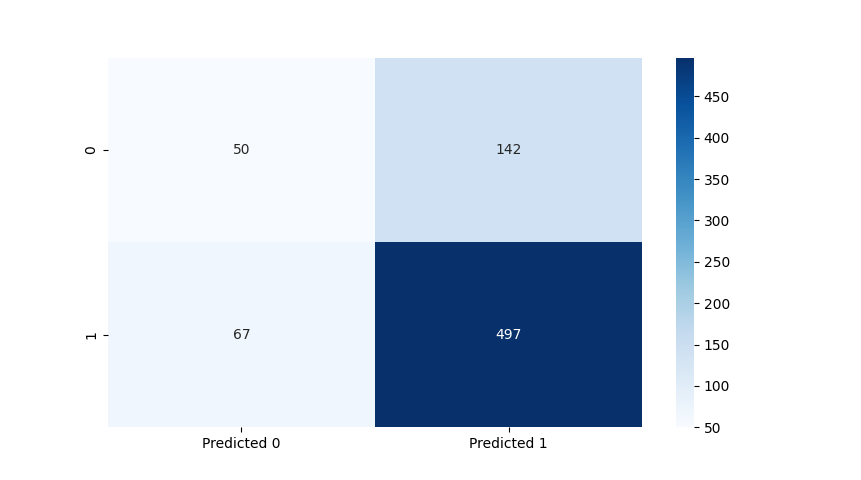
\includegraphics[width=1\linewidth,valign=t]{m1}
		      \caption{kNN Confusion Matrix}

		      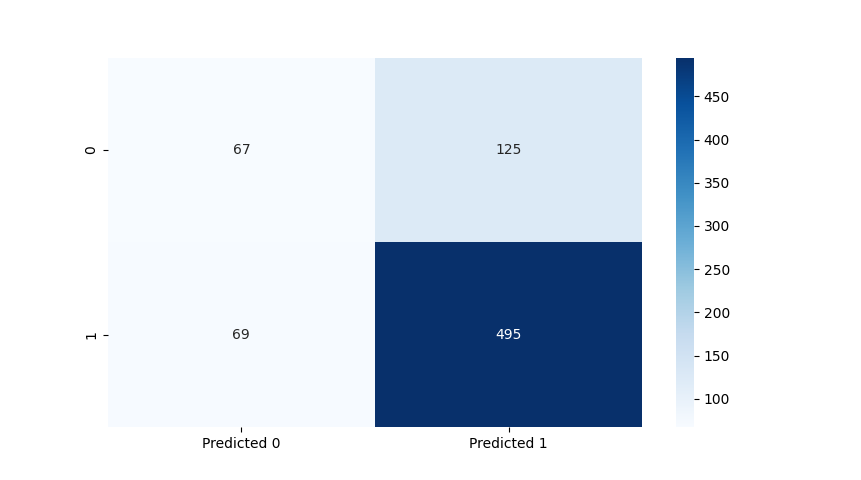
\includegraphics[width=1\linewidth,valign=t]{m2}
		      \caption{Naïve Bayes Gaussian Confusion Matrix}
	      \end{figure}

	\item
	      Defining $H_0$ as ``\emph{kNN is statistically superior to Naïve Bayes
		      regarding accuracy}" and $H_1$ as ``\emph{kNN is not statistically
		      superior to Naïve Bayes regarding accuracy}, the hypothesis test lead
	      to a p-value of $0.9104476998751558$. Therefore, we reject $H_0$,
	      concluding that kNN is not statistically
	      superior to Naïve Bayes regarding accuracy.

	\item
	      The Naïve Bayes classifier may have had better accuracy results due
	      to the small number of neighbours, $k$, of the kNN classifier, which
	      is known to have its accuracy increased as the value of $k$ rises.
	      The reduced dependence between the variables of the dataset favors
	      the Naïve Bayes classifier, which assumes variable independence,
	      increasing this classifier's accuracy. Furthermore, the Naïve Bayes
	      classifier is known to have better accuracy, compared to the kNN
	      classifier, when applied to big data.

\end{enumerate}

\pagebreak

\section{Appendix}
\lstinputlisting[language=Python]{./src/code.py}

\end{document}
